%%%%%%%%%%%%%%%%%%%%%%%%%%%%%%%%%%%%%%%%%%%%%%%%%%%%%%%%%%%%%%%%%%%%%%%
%% Zusammenfassung und Ausblick
\section{Entwicklung}
\label{sec:entwicklung}
Dieses Kapitel befasst sich mit einzelnen Aspekten der Entwicklung. Nach der anfänglichen Anforderungsanalyse werden grundlegende Konzepte und Architekturen vorgestellt. Dabei werden erste Sensoren, Aktoren und bestehende Software Bibliotheken getestet und für eine Anschlussverwendung bewertet. Die weiteren benötigten Softwarepaket werden im nachfolgenden Kapitel Implementierung umgesetzt.


\subsection{Anforderungen}
In diesem Kapitel werden die Anforderungen an das Robotersystem gestellt. Es werden die einzelnen Funktionalitäten für die Aktoren und Sensoren festgelegt. Außerdem werden die Anforderungen an die Architektur definiert. Das folgende Use-Case Diagramm \ref{fig:dev-usecase} stellt die groben Funktionsanforderungen an das Robotersystem dar.

 \begin{figure}[H]
 	\centering
 	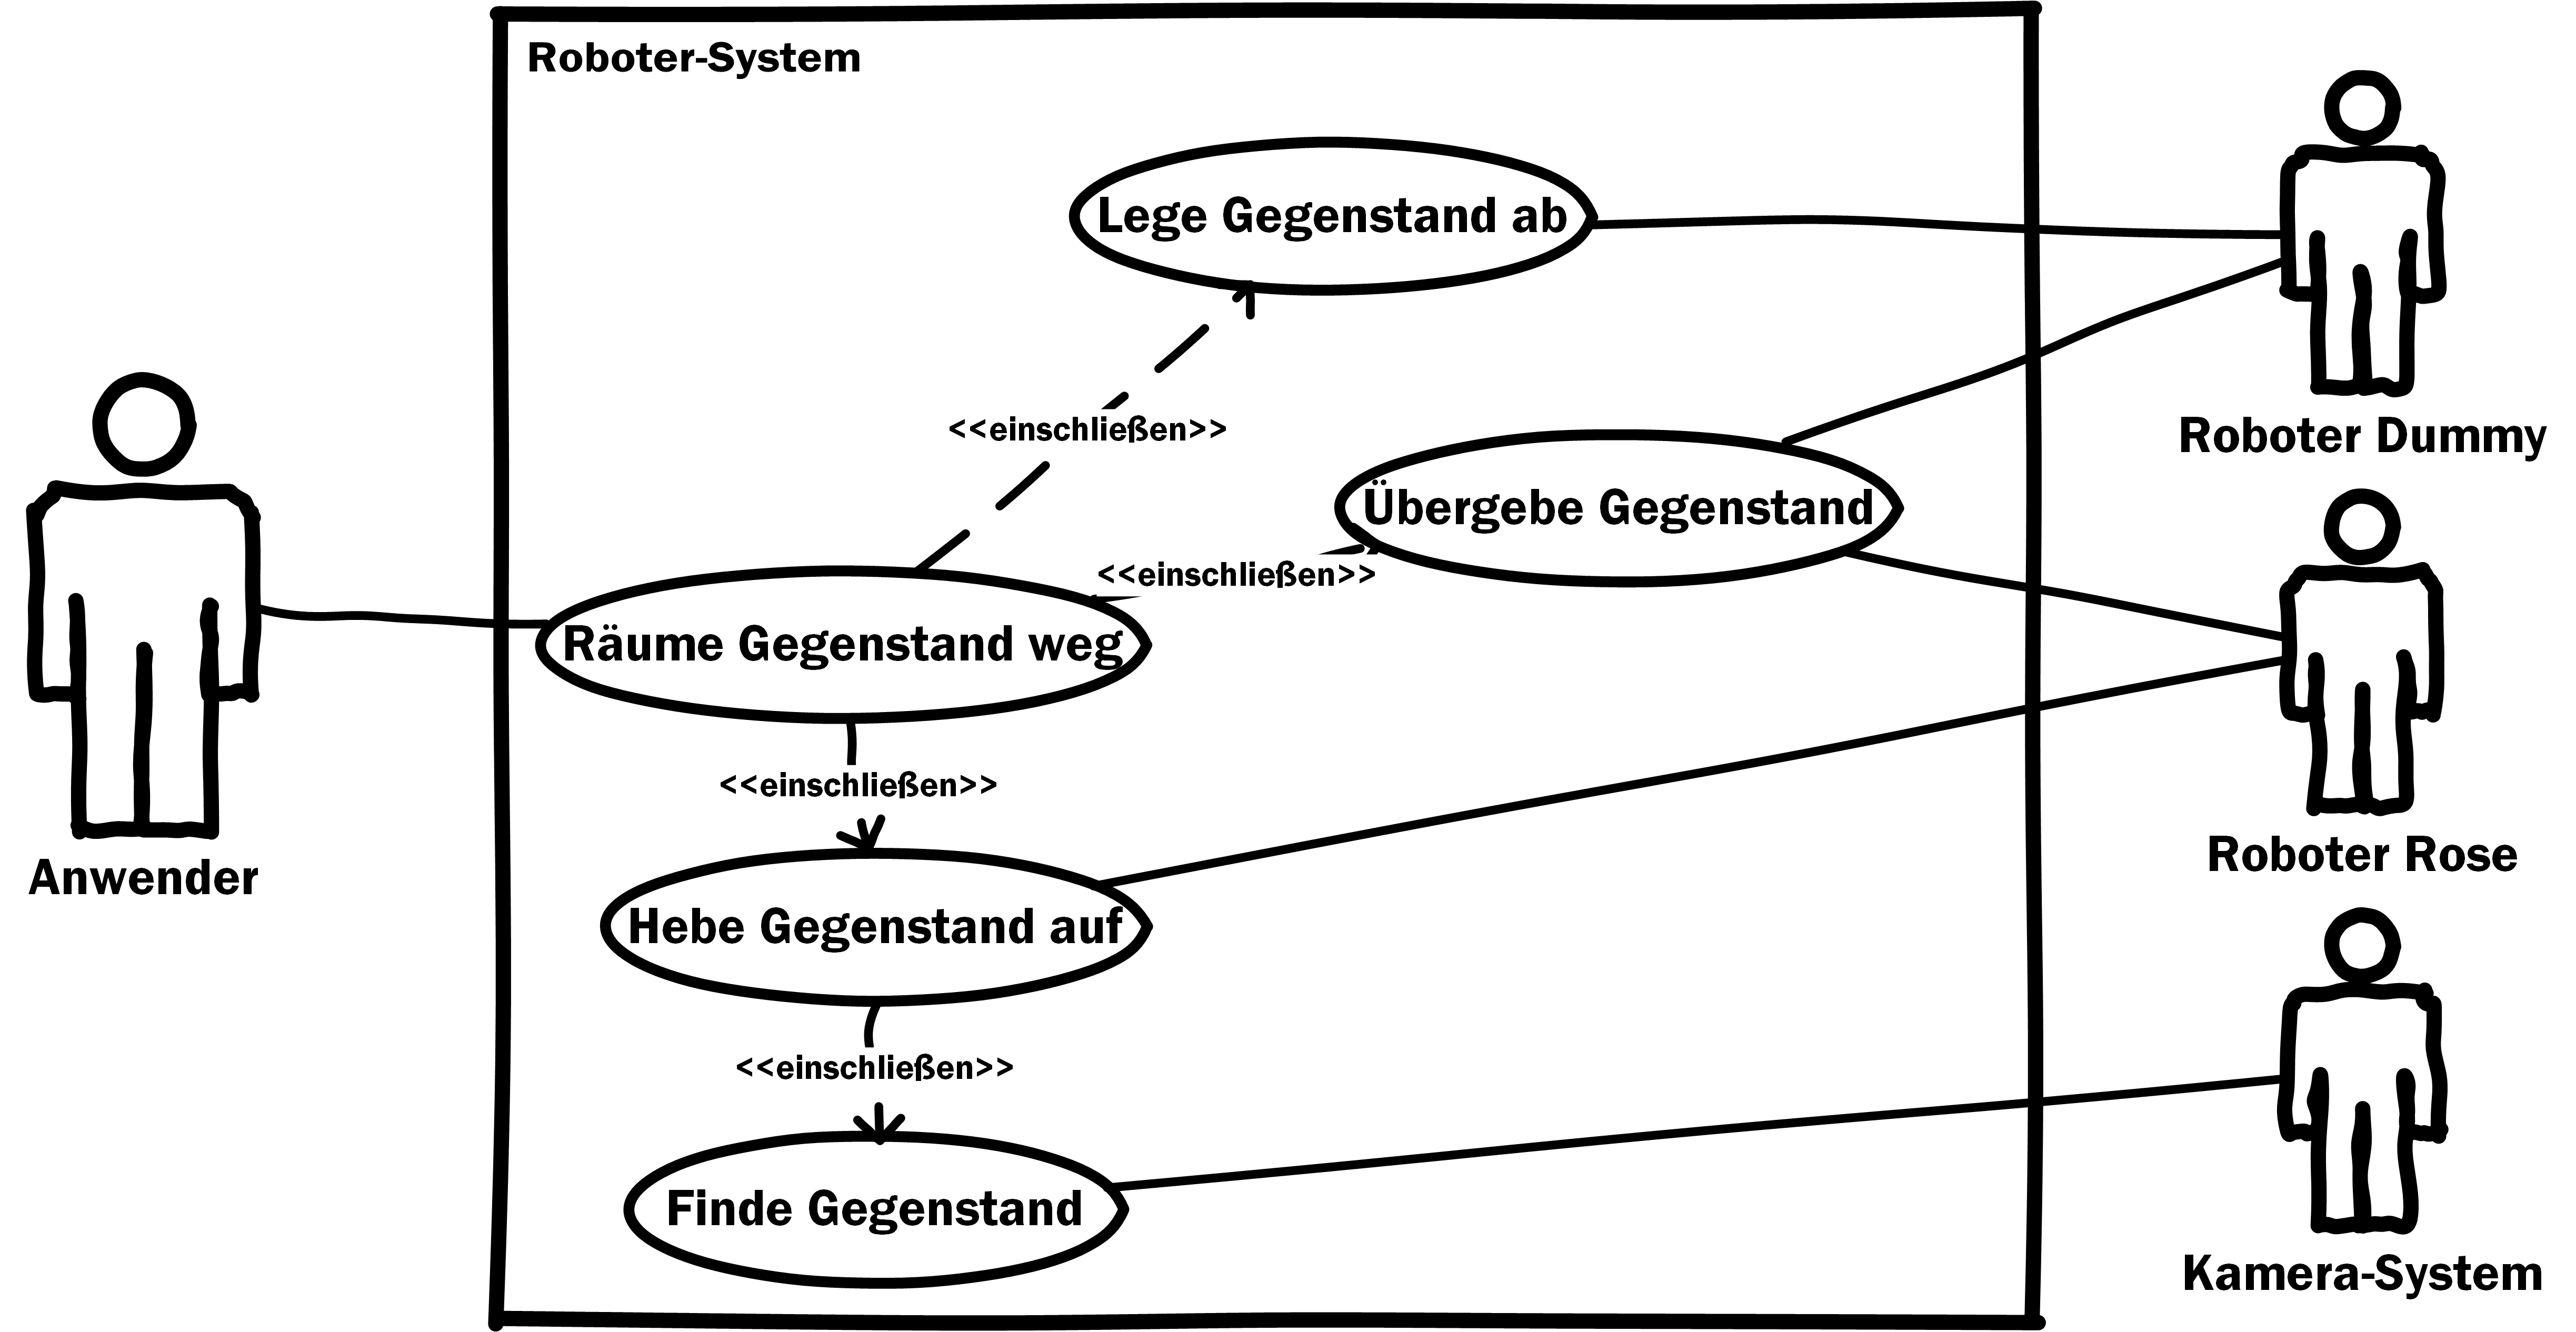
\includegraphics[scale=0.8]{fig/UseCase}   
 	\caption[Use-Case Robotersystem]{Vereinfachtes Use-Case Diagramm zur groben Funktionsübersicht des Robotersystems}
 	\label{fig:dev-usecase}
 \end{figure}
 
 Der Anwender gibt dem System die Anweisung einen Gegenstand wegzuräumen. Das Robotersystem gliedert die Anweisung in einzelne Tasks auf. Diese Tasks werden von den unterschiedlichen Akteuren mit ihren Funktionalitäten sequentiell oder parallel ausgeführt. In diesem konkreten Fall soll zunächst der Roboter Rose den entsprechenden Gegenstand aufheben. Dies erfordert zunächst eine Lokalisierung des Objektes die von einem Kamerasystem angefordert wird. Anschließend übergeben sich die Roboter Rose und Dummy den Gegenstand, bevor Dummy ihn anschließend an einer gewünschten Position ablegt. Diese sehr grobe Darstellung des Vorgangs beinhaltet die vier zentralen Funktionen, die das System umsetzen muss: Gegenstand aufheben (\textit{pick-up}), Gegenstand ablegen (\textit{place}), Gegenstand lokalisieren und Gegenstand übergeben(\textit{handover}). Des Weiteren muss es eine Möglichkeit für den Anwender geben Befehle an das System zu übergeben. Diese funktionalen Anforderungen werden im nächsten Unterkapitel \ref{sec:dev-funk} aufgelistet und definiert. Neben diesen funktionalen Anforderungen existieren noch nicht-funktionale Anforderungen. Zu diesen zählen Sicherheitsaspekte, sowie Anforderungen an die Zuverlässigkeit, Erweiterbarkeit und die Effizienz. Die nicht-funktionalen Anforderungen werden in Kapitel \ref{sec:dev-nichtfunk} aufgeführt. Die folgenden Anforderungen dienen zur Strukturierung der Arbeit und zerlegen das Robotersystem in Teilsysteme. Dies wird benötigt um einen Aufwand für die Koordinierung und Konfiguration zu bestimmen. Deshalb sind die Anforderungen grobe Darstellungen und aus dem Aspekt der Software-Entwicklung nicht detailliert genug. Dafür müssten die Funktionen weiter runter gebrochen werden. Dies würde jedoch den Umfang dieser wissenschaftlichen Arbeit überschreiten.
 
\subsubsection{Funktionale Anforderungen}
\label{sec:dev-funk}
Alle Funktionen werden nach dem Schema aus \cite{lundh2006plan} angegeben: 

$f = \langle  Id, r, I, O, \Phi, Pr, Po, Freq, Cost\rangle$

Jede Funktion $f$ entspricht dabei einem Tupel und ist einem oder mehreren Agenten im System zugewiesen. Diese Zuweisung wird im Feld $r$ in Kapitel TODO zugewiesen. Die weiteren Felder des Tupels stehen für:

\begin{description}
	\item [$Id$] Eindeutiger Bezeichner für die Funktion.
	\item [$I = \{i_1, i_2,\ldots,i_n\}$] Eine Menge aller Eingangsparameter.
	\item [$O = \{o_1, o_2,\ldots,o_n\}$] Eine Menge aller Ausgangsparameter.
	\item[$\Phi$] Definiert den Übergang zwischen Eingabe und Ausgabe.
	\item [$Pr$] Zustand $s \in S$ aus dem diese Funktion gestartet werden kann.
	\item [$Po : S \times I \rightarrow S$] Eine Funktion die den Folgezustand $s\textasciiacute$ anhand des Inputs und des Startzustandes $s$ angibt.
	\item[$Freq$] Frequenz in der die Funktionalität ausgeführt werden soll.
	\item[$Cost$] Kosten der Ausführung, zum Beispiel Zeit oder Energie. Können konstant aber auch funktionell angegeben werden.
\end{description}

Je nach Typ des Agenten sind die Eingabemenge bei Sensoren $I = \varnothing$ und die Ausgabemenge bei Aktoren $O =  \varnothing$. Außerdem wird jede Funktion beschrieben und für die Verwendung in ein MRS eingeordnet. Aus dem Anwendungsfall für das Robotersystem ergeben sich folgende funktionale Anforderungen.


\begin{tabular}{|p{3cm}|p{10cm}|}
	\multicolumn{2}{c}{	$f_0$ (Aufheben):}\\
	\hline  $Id$ & pickup\\ 
	\hline  $I$ & Objektposition im globalen oder lokalen Koordinatensystem. \\ 
	\hline  $O$ & Erfolgsmeldung. \\ 
	\hline  $\Phi$ & Wenn die Objektposition durch den Agenten erreichbar und der Agent voll funktionsfähig ist erfolgt eine positive Rückmeldung. Ansonsten eine negative Erfolgsmeldung.\\ 
	\hline $Pr$ & Zustand $s_1$, Objekt im Nahfeld gefunden und Arm in Candle-Stellung. \\ 
	\hline $Po$ & Zustand $s_2$, Arm in Candle-Stellung und Objekt gegriffen, oder Fehlerzustand $s_e$ bei Fehlschlag. \\ 
	\hline $Freq$ & Einmalige Funktion. \\ 
	\hline $Cost$ & Dynamisch zu ermitteln. Abhängig von Weg und Erreichbarkeit des Objektes. \\
	\hline
\end{tabular}

\paragraph{Beschreibung}
Die Funktion \textit{pickup} wird in den beiden Robotern Rose und Dummy implementiert und wird für das Aufheben von Objekten genutzt. Beschränkt wird diese Funktionalität durch die Erreichbarkeit der Objektposition. Gerade für den stationären Dummy ist der Arbeitsraum stark eingeschränkt. Rose hat die Möglichkeit während dieser Funktionalität die eigene Position zu verändern um das Objekt zu erreichen. Das Aufheben bedingt, dass das Objekt auf einer parallelen Ebenen zur X-Y-Ebene liegt, da die Greifer Z-Achse parallel zur globalen Z-Achse greift. Die Rotation um die Z-Achse des Objektes ist dabei frei wählbar, da diese durch eine Rotation des Greifers ausgeglichen werden kann. Damit der Roboter nicht auf dem Weg zum Objekt dasselbe berührt wird eine Position über dem Objekt angefahren, bevor der Greifer an der globalen Z-Achse hin abfährt.  Diese Beschränkung reduziert die Arbeitsräume der Roboterarme, da ein senkrechter Griff die Zahl der möglichen Gelenkpositionen stark einschränkt und jede Position auf dem senkrechten Pfad erreichbar sein muss. Eine nicht erreichbare Position führt zum Abbruch der Funktion. Eine anschließende sichere Konfiguration des Roboterarms ist nicht gewährleistet. Für Rose gilt des Weiteren auch ein undefinierter Standort nach Abbruch. Wird die Funktion erfolgreich beendet befindet sich der Arm in einer sicheren Konfiguration (\textit{Candle}- oder \textit{Fold}-Pose).

\paragraph{Einordnung}
Die Funktion ist als Single-Robot Task für einen Single-Task-fähigen Agenten einzuordnen, da nur ein Agent zur Erledigung nötig ist. Die Funktion kann von einem Multi-Task fähigen Agenten intern auch parallel ausgeführt werden, da einzelne Subtasks unabhängig von einander erledigt werden können. Ein Beispiel ist das Öffnen des Greifers während der Bewegungsphase des restlichen Armes oder der mobilen Plattform bei Rose. Diese Multi-Task Anwendung fordert aber einen höheren Koordinierungsaufwand, da Funktionen zeitlich voneinander abhängen (siehe TODO). Für eine Single-Task Anwendung ist der Koordinierungsaufwand gering, da alle Subtasks seriell ausgeführt werden. Der Konfigurationsaufwand ist mittel, da zwei Agenten für die Funktionalität bereitstehen, welche sich über den Aktionsradius für die Ausführung qualifizieren. 
 
\begin{tabular}{|p{3cm}|p{10cm}|}
	\multicolumn{2}{c}{$f_1$ (Ablegen):}\\
	\hline  $Id$ & place\\ 
	\hline  $I$ & Zielposition im globalen oder lokalen Koordinatensystem. \\ 
	\hline  $O$ & Erfolgsmeldung. \\ 
	\hline  $\Phi$ & Wenn die Zielposition durch den Agenten erreichbar und der Agent voll funktionsfähig ist erfolgt eine positive Rückmeldung. Ansonsten eine negative Erfolgsmeldung.\\ 
	\hline $Pr$ & Zustand $s_2$, Arm in Candle-Stellung und Objekt gegriffen. \\ 
	\hline $Po$ & Ruhezustand $s_r$, Arm in Candle-Stellung oder Fehlerzustand $s_e$ bei Fehlschlag. \\ 
	\hline $Freq$ & Einmalige Funktion.\\ 
	\hline $Cost$ & Dynamisch zu ermitteln. Abhängig von Weg und Erreichbarkeit der Zielpositionen. \\
	\hline
\end{tabular}

\paragraph{Beschreibung}
Ähnlich Funktion $f_0$ wird diese Funktionalität den beiden Robotern Dummy und Rose implementiert. Dabei legt der Arm ein Objekt an einer gewünschten Position ab. Beschränkt wird die Funktion auch durch den Arbeitsraum der einzelnen Roboter.  Das Objekt kann ebenfalls nur auf einer Ebene abgelegt werden, die parallel zur X-Y-Ebene ist. Die Rotation um die Z-Achse kann beim ablegen vorgegeben werden. im Gegensatz zu $f_0$ nähert sich der Greifer nicht dem Objekt an, sondern entfernt sich nach dem Ablegen positiv auf der globalen Z-Achse vom Objekt um dieses in einer anschließenden Bewegung nicht durch eine Berührung zu manipulieren. Bei einer erfolgreichen Ausführung beendet die Funktionalität befindet sich der Arm in einer sicheren Konfiguration (\textit{Candle}- oder \textit{Fold}-Pose). Bei einem Fehlschlag ist diese Konfiguration nicht garantiert.

\paragraph{Einordnung}
Die Funktion gilt als Single-Robot Task. Die Subtasks der Funktion können seriell als auch parallel ausgeführt werden. Dadurch eignen sie sich für Multi-Task, sowie Single-Task Agenten. Je nach Typ ist der Koordinierungsaufwand unterschiedlich hoch. Der Single-Task Agent benötigt wenig Koordinierung da nur ein Startsignal notwendig ist. Bei einem Multi-Task Agenten ist die Koordinierung aufwendiger, da Subtasks zeitlich voneinander abhängen. Zum Beispiel darf der Greifer erst öffnen, wenn das Objekt in der Position ist. Der Konfigurationsaufwand ist gering, da nur der Agent die Aktion ausführen kann, der den Gegenstand hält. 

\begin{tabular}{|p{3cm}|p{10cm}|}
	\multicolumn{2}{c}{$f_2$ (Objekt im Raum finden):}\\
	\hline  $Id$ & findObj\\ 
	\hline  $I$ & Gewünschte Objektdaten. \\ 
	\hline  $O$ & Position des Zielobjektes im globalen Koordinatensystem. \\ 
	\hline  $\Phi$ & Findet der Agent anhand der Objektdaten das Objekt wird die Position zurückgegeben. Ansonsten folgt eine Fehlermeldung.\\ 
	\hline $Pr$ & Ruhezustand $s_r$,Keine Vorbedingung nötig. \\ 
	\hline $Po$ & Zustand $s_0$, Objekt gefunden. Oder Fehlerzustand $s_e$\\ 
	\hline $Freq$ & Einmalige Funktion.\\ 
	\hline $Cost$ & Konstant. Abhängig von Prozessor der Recheneinheit, Algorithmus und Kamerasystem. \\
	\hline
\end{tabular} 

\paragraph{Beschreibung}
Diese Funktion identifiziert und lokalisiert ein bestimmtes Objekt im Großraum (Bodenfläche im Arbeitsraum größer als ein Quadratmeter). Je nach Typ der Identifizierung werden unterschiedliche Objektdaten benötigt. Eine Identifizierung basierend auf der Farbe des Objektes benötigt die Objektfarbe. Eine Identifizierung basierend auf der Form benötigt ein 3D-Modell oder eine Kostenfunktion für das Objekt. Die Identifizierung ist abhängig vom verwendeten Algorithmus. Dieser wird in TODO genauer erklärt. Findet die Funktion das gewünschte Objekt nicht oder tritt ein Fehler bei der Erkennung auf bricht die Funktion ab und gibt eine Fehlermeldung zurück. Bei einer erfolgreichen Identifizierung wird anhand von 3D-Daten die Position des Objektes berechnet. Bei dieser Lokalisierung soll eine Genauigkeit von fünf cm erreicht werden und damit nur eine grobe Position. Genauere Ergebnisse werden mit der Naherkennung $f_3$ erreicht. 

\paragraph{Einordnung}
Ein simpler Single-Robot Task, der von einem Agenten ausgeführt wird. Der Task wird in zwei Subtasks (Identifizieren und Lokalisieren) zerlegt, die serielle ausgeführt werden. Damit bringen Multi-Task Agenten keinen Vorteil. Der Koordinierungsaufwand ist sehr gering, da die Funktion nur angestoßen werden muss. Sollte die Funktion jedoch mit mehreren Kamerasystemen genutzt werden steigt der Koordinierungsaufwand, da der Task entweder parallel oder seriell von allen Systemen ausgeführt werden kann. Je nach Typ steigt der Konfigurationsaufwand, bei einer parallelen Ausführung ist kein Aufwand nötig, da immer alle Kamerasysteme genutzt werden. Eine serielle Ausführung würde die Komplexität steigen, da die Kamerasysteme in einer, möglicherweise priorisierten, Reihenfolge angestoßen werden.


\begin{tabular}{|p{3cm}|p{10cm}|}
	\multicolumn{2}{c}{$f_3$ (Nahfeld Erkennung):}\\
	\hline  $Id$ & findObjNear\\ 
	\hline  $I$ & Gewünschte Objektdaten. \\ 
	\hline  $O$ & Position des Zielobjektes im lokalen Koordinatensystem. \\ 
	\hline  $\Phi$ & Findet der Agent anhand der Objektdaten das Objekt wird die Position zurückgegeben. Ansonsten folgt eine Fehlermeldung.\\ 
	\hline $Pr$ & Zustand $s_0$, Objekt im Raum gefunden und im Arbeitsraum der Kamera. \\ 
	\hline $Po$ & Zustand $s_1$, Objekt im Nahfeld gefunden. Oder Fehlerzustand $s_e$\\ 
	\hline $Freq$ & Einmalige Funktion.\\ 
	\hline $Cost$ & Konstant. Abhängig von Prozessor der Recheneinheit, Algorithmus und Kamerasystem. \\
	\hline
\end{tabular} 

\paragraph{Beschreibung}
Diese Funktion identifiziert und lokalisiert ein bestimmtes Objekt im Nahfeld (Bodenfläche im Arbeitsraum kleiner als ein Quadratmeter). Es gelten die gleichen Merkmale wie bei $f_2$. Der verwendete Algorithmus wird in TODO genauer erklärt. Findet die Funktion das gewünschte Objekt nicht oder tritt ein Fehler bei der Erkennung auf bricht die Funktion ab und gibt eine Fehlermeldung zurück. Zusätzlich zur Position wird auch die Orientierung des Objektes berechnet. Die bestimmte Position entspricht dem Flächenschwerpunkt der Oberfläche des Objektes und soll eine Genauigkeit von fünf mm entsprechen.

\paragraph{Einordnung}
Wie $f_2$ einzuordnen. Kann jedoch nicht mit mehreren Kamerasystemen ausgeführt werden, da jedes Kamerasystem auf einem Roboter montiert und mit diesem eng-gekoppelt ist. Dadurch ist der Konfigurationsaufwand konstant, da jedem Roboter ein System zugewiesen wird. 

\begin{tabular}{|p{3cm}|p{10cm}|}
	\multicolumn{2}{c}{$f_4$ (Lokalisierung Agent):}\\
	\hline  $Id$ & loc\\ 
	\hline  $I$ & $\emptyset$ \\ 
	\hline  $O$ & Position des Agenten im globalen Koordinatensystem. \\ 
	\hline  $\Phi$ & Kann der Agent sich selbst im Raum lokalisieren, wird die Position zurückgegeben. Ansonsten folgt eine Fehlermeldung.\\ 
	\hline $Pr$ & In jedem Zustand $s_s$ möglich \\ 
	\hline $Po$ & Wie der Zustand beim Start $s_s$.\\ 
	\hline $Freq$ & Abhängig vom Sensor.\\ 
	\hline $Cost$ & Konstant. Abhängig von Prozessor der Recheneinheit, Algorithmus und Kamerasystem. \\
	\hline
\end{tabular} 

\paragraph{Beschreibung}
Diese Funktionalität lokalisiert den entsprechenden Agenten im Raum. Mögliche Algorithmen sind das Nutzen der Odometrie-Daten, bildbasierte Odometrie, bildbasierte Lokalisierung beruhend auf externen Sensoren und Funktionen ($f_2$) oder bildbasierte Lokalisierung basierend auf Merkmals-Erkennung. Es existieren noch weitere Methoden der Lokalisierung, dafür fehlen aber in dieser Arbeit die entsprechenden Sensoren und Aktoren.

\paragraph{Einordnung}
Eine an den Agenten enge-gekoppelte Funktionalität die an einen mobilen Roboter oder externen Sensor vergeben werden kann. Ein mobiler Roboter muss multi-tasking fähig sein, da diese Funktion in einer bestimmten Frequenz wiederholt wird und von anderen Funktionen benötigt wird. Ein Beispiel ist $f_0$, bei dieser Funktion benötigt Rose die eigene Position zur Fahrwegbestimmung. Dies erhöht den Grad der Koordinierung. Die Konfiguration ist je nach Algorithmus einfach bis komplex. Ein festmontierter Sensor auf einer mobilen Plattform benötigt eine einmalige Konfiguration. Externe Sensoren, zum Beispiel Kamerasysteme, benötigen eine größeren Konfigurationsaufwand. Da zunächst das Kamerasystem ausgewählt werden muss in dessen Arbeitsraum sich der gesuchte Agent befindet. Dadurch steigt auch der Koordinierungsaufwand.

\begin{tabular}{|p{3cm}|p{10cm}|}
	\multicolumn{2}{c}{$f_5$ (Übergabe Objekt):}\\
	\hline  $Id$ & handover\\ 
	\hline  $I$ & $\emptyset$ \\ 
	\hline  $O$ & $\emptyset$ \\ 
	\hline  $\Phi$ & Bei Fehlschlag erfolgt Fehlermeldung.\\ 
	\hline $Pr$ & Aus Zustand $s_2$ möglich. Ein Objekt wurde gegriffen.  \\ 
	\hline $Po$ & Endet in Zustand $s_2$. Im Gegensatz zu $Pr$ befindet sich das Objekt im Greifer des anderen Roboters. Bei Fehlschlag endet die Funktion in $s_e$.\\ 
	\hline $Freq$ & Einmalig.\\ 
	\hline $Cost$ & Dynamisch. Abhängig von der Distanz zwischen den beiden Akteuren und der benötigten Bewegungen der Arme. \\
	\hline
\end{tabular} 

\paragraph{Beschreibung}
Diese Funktionalität bildet die zentrale Aufgabe dieser Arbeit ab. Ein Objekt soll zwischen zwei Robotern übergeben werden. Roboter A hat das Objekt gegriffen und soll nun dieses nur an Roboter B übergeben. Dazu müssen zunächst die beiden Arbeitsräume der Roboter eine Schnittmenge aufweisen in der das Objekt übergeben werden kann. Danach muss eine Übergabeposition bestimmt werden. Diese sollte möglichst Energieeffizient sein. Neben der Position spielt die Orientierung im Raum einen wichtigen Faktor, da je nach Objekt und Greifer die Griffpositionen an dem Objekt variiert. Da in dieser Arbeit mit einem einfachen symmetrischen Objekt, einem langgezogenen Quader, und einem Gripper mit parallelen Fingern gearbeitet wird, ist ein entgegengesetzter Griff möglich. Dabei entspricht die Pose von Greifer B der invertierten Pose von Greifer A:

\begin{equation}
\xi_{GreiferB} = \ominus \xi_{GreiferA}
\label{eq:grip}
\end{equation}


Neben der Greifposition ist auch die Pfadplanung zur Greifposition wichtig, da der sich nähernde Greifer weder mit dem Objekt noch mit dem anderen Greifer kollidieren darf. Ebenfalls kann die Symmetrie der Übergabe genutzt werden. Unter der Bedingung, dass die Finger von Greifer A nicht die selbe Position haben dürfen wie die Finger von Greifer B, muss die Gleichung \ref{eq:grip} um ein Offset $\xi_\tau$ entlang der X-Achse des Objekts erweitert werden. Die Länge des Offsets $|\tau|$ entspricht dabei der Hälfte der aufsummierten Breiten der Finger der Greifer.

\begin{equation}
\xi_{GreiferB} = \ominus \xi_{GreiferA} \oplus \xi_\tau
\label{eq:grip2}
\end{equation}



\paragraph{Einordnung}
Diese Funktion ist eng-gekoppelt und benötigt einen hohen Aufwand an Koordinierung. Neben der Übergabeposition und -orientierung müssen auch die Zeitvorgaben für das Öffnen und Schließen der Greifer, sowie die Bewegungen koordiniert werden. 

\subsubsection{Nicht-Funktionale Anforderungen}
\label{sec:dev-nichtfunk}


\subsection{Architektur RATS}
\subsection{Sensoren und Aktoren}
\subsection{Inverse Kinematik}

